%; whizzy paragraph -pdf xpdf -latex ./whizzypdfptex.sh
%; whizzy-paragraph "^\\\\begin{frame}\\|\\\\emtext"
% latex beamer presentation.
% platex, latex-beamer $B$G%3%s%Q%$%k$9$k$3$H$rA[Dj!#(B 

%     Tokyo Debian Meeting resources
%     Copyright (C) 2012 Junichi Uekawa

%     This program is free software; you can redistribute it and/or modify
%     it under the terms of the GNU General Public License as published by
%     the Free Software Foundation; either version 2 of the License, or
%     (at your option) any later version.

%     This program is distributed in the hope that it will be useful,
%     but WITHOUT ANY WARRANTY; without even the implied warreanty of
%     MERCHANTABILITY or FITNESS FOR A PARTICULAR PURPOSE.  See the
%     GNU General Public License for more details.

%     You should have received a copy of the GNU General Public License
%     along with this program; if not, write to the Free Software
%     Foundation, Inc., 51 Franklin St, Fifth Floor, Boston, MA  02110-1301 USA

\documentclass[cjk,dvipdfm,12pt]{beamer}
\usetheme{Tokyo}
\usepackage{monthlypresentation}

%  preview (shell-command (concat "evince " (replace-regexp-in-string "tex$" "pdf"(buffer-file-name)) "&")) 
%  presentation (shell-command (concat "xpdf -fullscreen " (replace-regexp-in-string "tex$" "pdf"(buffer-file-name)) "&"))
%  presentation (shell-command (concat "evince " (replace-regexp-in-string "tex$" "pdf"(buffer-file-name)) "&"))

%http://www.naney.org/diki/dk/hyperref.html
%$BF|K\8l(BEUC$B7O4D6-$N;~(B
\AtBeginDvi{\special{pdf:tounicode EUC-UCS2}}
%$B%7%U%H(BJIS$B7O4D6-$N;~(B
%\AtBeginDvi{\special{pdf:tounicode 90ms-RKSJ-UCS2}}

\title{$BEl5~%(%j%"(BDebian$BJY6/2q(B}
\subtitle{$BBh(B93$B2s(B 2012$BG/(B10$B7nEY(B}
\author{$B>e@n=c0l(B\\dancer@debian.org}
\date{2012$BG/(B10$B7n(B20$BF|(B}
\logo{\includegraphics[width=8cm]{image200607/openlogo-light.eps}}

\begin{document}

\frame{\titlepage{}}

\begin{frame}{$B@_1D=`Hw$K$46(NO$/$@$5$$!#(B}
$B2q>l@_1D$h$m$7$/$*$M$,$$$7$^$9!#(B
\end{frame}

\begin{frame}{Agenda}
\begin{minipage}[t]{0.45\hsize}
  \begin{itemize}
  \item $BCm0U;v9`(B
	\begin{itemize}
	 \item $B0{?)6X;_(B
	 \item $B=!656X;_(B
	 \item $B1DMx3hF06X;_(B
	\end{itemize}
   \item $B:G6a$"$C$?(BDebian$B4XO"$N%$%Y%s%HJs9p(B
	\begin{itemize}
        \item $BBh(B91$B2s(B $BEl5~%(%j%"(BDebian$BJY6/2q(B
        \item $BBh(B0$B2s(BDebian$B%Q%C%1!<%8%s%0F;>l(B
	\end{itemize}
   \item DWN quiz
   \item $B;vA02]Bj>R2p(B
 \end{itemize}
\end{minipage} 
\begin{minipage}[t]{0.45\hsize}
 \begin{itemize}
  \item Haskell $B$N(B Debian packaging $B<~JU$K$D$$$F8l$j$^$9(B
  \item $B%l%4$G$J$a$3<}3O4|(B
  \item xf86-input-mtrack

 \end{itemize}
\end{minipage}
\end{frame}


\section{DWN quiz}
\emtext{DWN quiz}
\begin{frame}{Debian $B>o<1%/%$%:(B}

Debian $B$N>o<1!"$b$A$m$sCN$C$F$^$9$h$M(B?
$BCN$i$J$$$J$s$FCQ$:$+$7$/$F!"CN$i$J$$$H$O8@$($J$$$"$s$J$3$H$d$3$s$J$3$H!"(B
$B$_$s$J$G3NG'$7$F$_$^$7$g$&!#(B

$B:#2s$N=PBjHO0O$O(B\url{debian-devel-announce@lists.debian.org},
\url{debian-devel@lists.debian.org} $B$KEj9F$5$l$?(B
$BFbMF$H(BDebian Project News$B$J$I$+$i$G$9!#(B

\end{frame}

\subsection{$BLdBj(B}
%; whizzy-master ../debianmeetingresume201210.tex
% $B0J>e$N@_Dj$r$7$F$$$k$?$a!"$3$N%U%!%$%k$G(B M-x whizzytex $B$9$k$H!"(Bwhizzytex$B$,MxMQ$G$-$^$9!#(B
%

\santaku
{9/29 $B$K9T$o$l$?(B Debian 6.0 $B$N%"%C%W%G!<%H$O2?2sL\$G$7$g$&$+!#(B}
{5}
{6}
{7}
{B}
{6.0.6 $B$G$9!#(B}

\santaku
{DMUA $B%U%#!<%k%I$,$J$/$J$j!"(BDebian Maintainer$B$N%"%C%W%m!<%I$,JQ99$5$l$^$9!#:#8e!"%"%C%W%m!<%I$N:]$K$I$N$h$&$K:n6H$9$kI,MW$,$"$k$+!)(B}
{FTP master$B$KEEOC(B}
{$B%9%]%s%5!<$K(B dak $B$N=hM}$r0MMj$9$k(B}
{$B@lMQ%"%C%W%m!<%@$K%"%C%W%m!<%I(B}
{B}
{}

\santaku
{IRC $B7PM3$G(BVCS $B%j%]%8%H%j$r4F;k$9$k%5!<%S%9$G=*N;$7$?$b$N$O!)(B}
{ICPO}
{NPA}
{CIA}
{C}
{KGB$B$K0\9T!#(BICPA:  International Criminal Police Organization, NAP:National Police Agency, CIA: Central Intelligence Agency}

\santaku
{Debian Policy $B%a%s%F%J$K?7$7$/F~$C$?$N$OC/$+!)(B}
{Kei Hibino}
{Colin Watson}
{Charles Plessy}
{C}
{Andrew McMillan, Colin Watson, Manoj Srivastava $B$,H4$1$?(B}

\santaku
{Checksums-SHA1,SHA256 $B$N<h$j07$$$,JQ99$K$J$C$?$,!"$I$&JQ99$5$l$?$+!)(B}
{$B:#$^$GL5;k$5$l$F$$$^$7$?!#$4$a$s$M!#(B}
{$B%*%W%7%g%s$@$C$?$N$G!"I,?\$H$7$^$7$?!#(B}
{$B$3$l$i$OGQ;_$7!"(BSHA-512$B$N$_$K$7$^$9!#(B}
{B}
{Bug\#690293}



\emtext{$B;vA02]Bj(B}
{\footnotesize
 

\begin{prework}{ $B4d>>(B $B?.MN(B }

(1) erlang $B$H(BHaskell $B$r>/!9!#(B

(2) Real World Haskell$B!#%W%m%0%i%_%s%0(BErlang$B!#(B

(3) Erlang $B$N(B $B%S%k%I%7%9%F%`$G$"$k(B rebar $B$r$b$&$A$g$C$HM}2r$7$?$$!#(B


\end{prework}

\begin{prework}{ yamamoto }

(1) $B4X?t7?%W%m%0%i%_%s%08@8l$NMxMQ7P83(B $B!](B $B$J$7(B
(2) $B$*4+$a=q@R(B $B!](B $BFI$s$@$3$H!"$"$j$^$;$s(B
(3) $B;H$C$F$_$?$$%=%U%H(B $B!](B $BFC$K$J$7(B

$B$G$b!"(Bhaskell $B$O$J$s$+LLGr$=$&$@$7!"3X$s$G$_$h$&$+$J!)$H$+9M$($F$$$^$9!#(B
\end{prework}

\begin{prework}{ alice.ferrazzi }


\end{prework}

\begin{prework}{ $BNkLZ?rJ8(B }

(1)Debian $B$G$N4X?t7?%W%m%0%i%_%s%08@8l$NMxMQ7P83$H$=$N;~$K46$8$?;vJA!J(BLisp, Emacs Lisp, OCaml, Haskell $BEy!K(B
Erlang $B!&!&!&$5$o$jDxEY$G$9$,!"(BRiak$B$J$I$N<BMQ%l%Y%k$N%=%U%H%&%'%"$G;HMQ$5$l$F$$$kE@$d!"J,;64D6-$dL5Dd;_$K8@8l%l%Y%k$GBP1~$5$l$F$$$kE@$,LLGr$+$C$?$G$9!#(BRiak$B$+$i>pJs$r<h$C$?$jF~$l$?$j$9$k$@$1$J$i$PHf3SE*4JC1$KA`:n$G$-$^$7$?!#(B
Haskell $B!&!&!&$5$o$jDxEY$G$9$,!"(BHaskell$B9%$-$J?M$,B?$$$?$a3X$V$K$ONI$$8@8l$@$H46$8$^$7$?!#(B

(2) $B4X?t7?%W%m%0%i%_%s%08@8l=i?4<T$K8~$1$?$*4+$a=q@R$H$=$N%&%j$N>R2p(B
Erlang$B$O$J$+$J$+K\$,$J$+$C$?$G$9!#(BHaskell$B$O!V$9$4$$(BHaskell$B$?$N$7$/3X$\$&!*!W$,FI$_$d$9$$$h$&$K46$8$^$9$,!"$^$@M}2r$G$-$F$^$;$s!#(B

(3) $B4X?t7?8@8l$G<BAu$5$l$F$$$k!";H$C$F$_$?$$%=%U%H$r$"$2$F$/$@$5$$(B
Riak
xmonad

\end{prework}

\begin{prework}{ $B5HLn(B(yy_y_ja_jp) }

(1) $B:G6a(BHaskell$B$r?($C$F$$$^$9!%(Bcabal-debian$B$r$b$&>/$7CN$j$?$$$G$9!%(B
\end{prework}

\begin{prework}{ $B%-%?%O%i(B }

(1) Haskell $BF~Lg=q$N%5%s%W%k$rF0$+$7$?DxEY!"(B
    apt-get$B$G4JC1$KF3F~$G$-$F46F0$7$?$h$&$J5-21$,!&!&!&!#(B
(2) Haskell$B$NF~Lg=q$r(B2$B:}$[$IFI$_$^$7$?$,!"6&$K(Bmonad$B$G(B
    $B:C@^$7$?!":G6a$NK\$OFI$s$G$$$J$$!#(B
(3) $BFC$K$J$7!#(B

\end{prework}

\begin{prework}{ dictoss($B?yK\!!E5=<(B) }

(1) emacs.el$B$r=q$/$/$i$$$G$J$s$H$J$/;H$C$F$$$k46$8$G$9!#%7%s%0%k%/%)!<%F!<%7%g%s$OJD$8$J$/$F$$$$>l9g$,$"$k$N$G$=$l$K8MOG$&$3$H$,$"$j$^$9!#(B
\end{prework}

\begin{prework}{ $BLn<s(B }

elisp$B$G$A$g$C$H(Bmajor mode$B$H(Bshinbum module$B$r=q$$$F$_$?$3$H$,$"$k$0$i$$$G$9!#(B
$B4X?t7?%W%m%0%i%_%s%0$H$$$&%l%Y%k$K;j$j$^$;$s$G$7$?!#(B

\end{prework}

\begin{prework}{ @Lost_dog_ }

 (1) Haskell:$B7?0BA4$N$"$j$,$?$_$,J,$+$C$?(B
 (2) $B!X$9$4$$(BHaskell$B$?$N$7$/3X$\$&(B!$B!Y$O4X?t7?$NJ70O5$$rPmbW$G$-$k!#K\5$$GJY6/$9$k$J$i!"$b$C$H2&F;$N%F%-%9%H$rA*$s$@$[$&$,$h$$$+$b!#(B
 (3) yi-editor
\end{prework}

\begin{prework}{ $BF|HfLn(B $B7<(B }

(1) Haskell, OCaml $B$H$b$K(B Debian $B$K$OB??t$N%Q%C%1!<%8$,$"$C$F$9$P$i$7$$$G$9!#(B

(2)
\begin{itemize}
\item {\bf $B%W%m%0%i%_%s%0(BHaskell\\ - Graham Hutton ($BCx(B), $B;3K\(B $BOBI'(B ($BK]Lu(B)]}\\
$B:G=i$KFI$`$J$i$3$l$G$9!#4X?t%W%m%0%i%_%s%0$N%H%T%C%/$rJ?0W$K2r@b$7$J$i$,(BHaskell$B$r;n$7$F$$$-$^$9!#(B
\item {\bf $B$9$4$$(BHaskell$B$?$N$7$/3X$\$&(B!\\ - Miran Lipovaa ($BCx(B), $BEDCf(B $B1Q9T(B ($BK]Lu(B), $BB<<g(B $B?r9T(B ($BK]Lu(B)}\\
$B!V%W%m%0%i%_%s%0(BHaskell$B!W$N<!$O$3$l$@$H;W$$$^$9!#$h$jJ#;($J7?$N5!G=$r$b4^$a$F(BHaskell$B$N2r@b$,?J$s$G$$$-$^$9!#(B
\item {\bf Real World Haskell $B<B@o$G3X$V4X?t7?8@8l%W%m%0%i%_%s%0(B\\
 - Bryan O'Sullivan ($BCx(B), John Goerzen ($BCx(B), Don Stewart ($BCx(B), $B;32<(B $B?-IW(B ($BK]Lu(B), $B0KEl(B $B>!Mx(B ($BK]Lu(B), $B3t<02q<R%?%$%`%$%s%?!<%a%G%#%"(B ($BK]Lu(B)}\\
$B<B:]$K(BHaskell$B$r8=>l$GMxMQ$7$F$k?M$?$A$,=q$$$?K\$H$7$F$N2ACM$,$"$kK\$G$9!#(B
Haskell$B$K$b$$$m$$$m$J%i%$%V%i%j$,$"$j!"$=$NMxMQNc$H$7$F;29M$K$J$k$H;W$$$^$9!#(B
$B>/$78E$$$N$,LdBjE@$G$9!#(B
\end{itemize}

(3) OCaml$B$G:n$i$l$F$$$kDjM}>ZL@4o(BCoq$B$r$&$^$/;H$($k$h$&$K$J$j$?$$$G$9!#$"$H(BHaskell$B$G$$$m$$$m:n$kB&$K$^$o$j$?$$!#(B

\end{prework}

}

\emtext{xf86-input-mtrack}

\begin{frame}{xf86-input-mtrack}

\begin{itemize}
\item $B@N$N(B Macbook \\
pre-multitouch$B%5%]!<%H(B
\item $B:G6a$N(B Macbook Pro / Air /Magic Trackpad\\
$B%^%k%A%?%C%A%5%]!<%H!#(B\\
$B:G=i$O(B synaptics $B%I%i%$%P$G$OF0:n$7$^$;$s$G$7$?!#(B\\
xserver-xorg-input-mrack / multitouch $B$r;H$&I,MW$,$"$j$^$9!#(B
\end{itemize}

\end{frame}


\begin{frame}{synaptics $B$H(B mtrack}
\begin{itemize}
\item synaptics $B$G$O!"%W%m%H%3%k(BA $B$N$_$N%5%]!<%H!J$@$C$?!)!K(B\\
$B$3$l$O%?%C%A(BID$B$r;}$C$F$$$J$$$?$a!"%H%i%C%-%s%0%3%s%?%/%H$r4IM}$G$-$^$;$s!#(B
%$B%9%F!<%H%l%9(B
%$B%9%F!<%H%U%k(B

\item mtrack $B$G$O!"%?%C%A(BID$B$r%5%]!<%H$7$?%W%m%H%3%k(BB $B$r%5%]!<%H!#(B
$B$3$l$K$h$j!"$h$j:Y$+$$%?%C%A%Q%C%I$N@)8f$,$G$-$k$h$&$K$J$C$F$$$^$9!#(B

\item Macbook Pro$BEy$KEk:\$5$l$F$$$k(B BCM5974 $B$N5!G=$r%5%]!<%H$7$F$$$^$9!#(B\\
\end{itemize}

\end{frame}

\begin{frame}

\begin{itemize}
\item $B$^$?!"!V%W%m%H%3%k(BB$B!W$r(BLinux$B%+!<%M%k$+$i<u?.$7!"$=$l$r(BX$B%I%i%$%P$K$o$+$j$d$9$$(B
$B!J?M4V$K$H$C$F$o$+$j$d$9$$!K7A$K%G!<%?$r7A@.$9$k%i%$%V%i%j(B mtdev $B$r(B
$B;H$$$^$9!#(B
\end{itemize}
\begin{center}
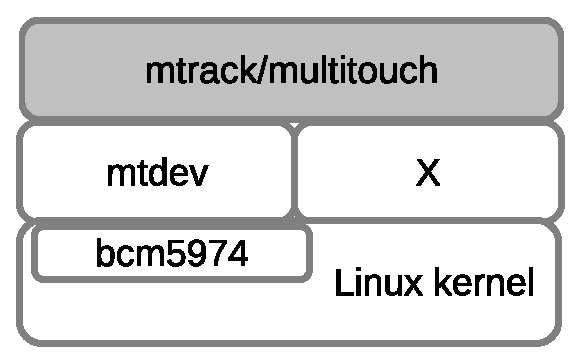
\includegraphics[width=0.5\hsize]{image201210/mtrack.eps}
\end{center}

\end{frame}

\begin{frame}[containsverbatim]

$B%W%m%H%3%k(BA
\begin{minipage}[t]{0.4\hsize}
\begin{commandline}
ABS_MT_POSITION_X x[0]
ABS_MT_POSITION_Y y[0]
SYN_MT_REPORT
ABS_MT_POSITION_X x[1]
ABS_MT_POSITION_Y y[1]
SYN_MT_REPORT
SYN_REPORT
\end{commandline}
\end{minipage}

$B%W%m%H%3%k(BB
\begin{minipage}[t]{0.4\hsize}
\begin{commandline}
ABS_MT_SLOT 0
ABS_MT_TRACKING_ID 45
ABS_MT_POSITION_X x[0]
ABS_MT_POSITION_Y y[0]
ABS_MT_SLOT 1
ABS_MT_TRACKING_ID 46
ABS_MT_POSITION_X x[1]
ABS_MT_POSITION_Y y[1]
SYN_REPORT
\end{commandline}
\end{minipage}

\end{frame}

\begin{frame}{multitouch $B$H(B mtrack}

\begin{itemize}
\item multitouch\\
$B4pK\E*$J@_Dj(B
\item mtrack\\
multitouch $B$+$i$N%U%)!<%/!#(B\\
$B:Y$+$$5!G=$N%5%]!<%H!#(B\\
\end{itemize}

\end{frame}

\begin{frame}[containsverbatim]{Debian $B$G;H$&(B}

\begin{itemize}
\item Debian $B$G$O4{$K%Q%C%1!<%82=$5$l$F$*$j!"(BAPT $B$G%$%s%9%H!<%k$G$-$^$9!#(B

\begin{commandline}
$ sudo apt-get install xserver-xorg-input-mtrack
\end{commandline}
%$
\end{itemize}

\end{frame}

\begin{frame}[containsverbatim]{$B%G%U%)%k%H$N@_Dj(B}

\begin{commandline}
Section "InputClass"
    MatchIsTouchpad "true"
    Identifier "Multitouch Touchpad"
    Driver "mtrack"
EndSection
\end{commandline} 

\end{frame}

\begin{frame}[containsverbatim]
$B%$%s%9%H!<%k$7$?CJ3,$G$O!"%G%U%)%k%H$N@_Dj$GF0:n$7$^$9!#(B
$B:Y$+$$@_Dj$r9T$&$?$a$KB?$/$N9`L\$,$"$j$^$9!#(B
\begin{table}[htb]
  \begin{tabular}{llc}
    $B9`L\(B & $BFbMF(B & $B%G%U%)%k%HCM(B \\
    TrackpadDisable & $B%H%i%C%/%Q%C%I5!G=$NF0:nFbMF$HL58z2=(B & 0 \\
    Sensitivity & $B%H%i%C%/%Q%C%I$N%9%T!<%I(B & 1 \\
    FingerHigh & $B;X$,%?%C%A$H$7$F8!CN$5$l$k05NO(B & 5 \\
    FingerLow & $B;X$,%j%j!<%9$H$7$F8!CN$5$l$k05NO(B & 5 \\
    IgnoreThumb & $B?F;X$G$"$k$H$o$+$k%?%C%A$rL5;k$9$k$+(B & False \\
    IgnorePalm & $B<j$NJ?$G$"$k$H$o$+$k%?%C%A$rL5;k$9$k$+(B & False \\
    DisableOnThumb & $B?F;X$,$5$o$C$F$$$k$H$-A4$F$N%H%i%C%/%Q%C%I$rL58z$K$9$k$+(B & False \\
    DisableOnPalm & $B<j$NJ?$,$,$5$o$C$F$$$k$H$-A4$F$N%H%i%C%/%Q%C%I$rL58z$K$9$k$+(B & False \\
    ThumbRatio & $B?F;X$NI}(B/$BD9HfN((B & 70 \\
    ThumbSize & $B?F;X$N:G>.8B$N%5%$%:(B & 25 \\
    PalmSize & $B<j$NJ?$N:G>.8B$N%5%$%:(B & 10 \\
  \end{tabular}
\end{table}
.......

\end{frame}

\begin{frame}[containsverbatim]{$BM-8z$J@_Dj(B}

$B%H%i%C%/%Q%C%I$N%7%s%0%k%?%C%W$rL58z$K$9$k(B\\
$B%H%i%C%/%Q%C%I$K?($C$F$b!J%7%s%0%k%?%C%W$7$F$b!K2?$b5/$-$J$/$J$j$^$9!#(B

\begin{commandline}
Option "TapButton1" "0"
Option "TapButton2" "0"
Option "TapButton3" "0"
\end{commandline}

\end{frame}

\begin{frame}[containsverbatim]{$BM-8z$J@_Dj(B}

$B#2K\;X%9%/%m!<%k$NF0$-$r$r(BOS X$B$HF1$8$K$9$k(B
\begin{commandline}
Option "ScrollUpButton" "5"
Option "ScrollDownButton" "4"
\end{commandline}

\end{frame}

\begin{frame}[containsverbatim]{$B$=$NB>$N>pJs(B}

\begin{itemize}

\item $B8=:_$N(B mtrack $B%I%i%$%P$O(B synaptics $B$N$h$&$K@_DjCM$rF0E*$KJQ99$G$-$^$;$s!#(B

\item $B$3$l$G$O:Y$+$$@_DjEy$r9T$&;~$KBgJQ$J$N$G>o$K@_Dj$rJQ99$G$-$k$h$&$K$9$k$?$a$N%Q%C%A$r(B
$B:n@.$7!"%"%C%W%9%H%j!<%`$KAw$j$^$7$?!#(B
\url{https://github.com/BlueDragonX/xf86-input-mtrack/pull/41}

$B%Q%C%A$rE,MQ$7!"0J2<$N@_Dj$r9T$J$C$F(BX$B%5!<%P$rN)$A>e$2$k$H(B
$BF0E*$K@_Dj$rJQ99$G$-$k$h$&$K$J$j$^$9!#(B
\begin{commandline}
Option "SHMConfig" "true"
\end{commandline}

\end{itemize}

\end{frame}

\begin{frame}{$B@_Dj%D!<%k(B}

$B4N?4$N@_DjMQ$N%D!<%k$G$9$,!"E,Ev$K:n$C$?$N$G8eF|8x3+$7$^$9!#(B

\end{frame}

\begin{frame}{$B%G%b(B}

\end{frame}

\begin{frame}{Debian$B$G%^%k%A%?%C%A$r;H$&>l9g$K$O$I$&$7$?$i$$$$$N$+(B}

\begin{itemize}
\item $BBgE}0l(BDebian$BJY6/2q$G$N@VIt$5$s$NH/I=(B\footnote{\url{http://gum.debian.or.jp/download/debian-gum-presentation.akabe.pdf}}
$B$K$b$"$C$?$h$&$K!"(BDebian $B$G$O$^$@%^%k%A%?%C%A$r(B
$BDs6!$9$k%D!<%kEy$,==J,$G$O$"$j$^$;$s!#(B

\item X $B$d(B GTK+ $B$J$I$G$O4{$K%^%k%A%?%C%A$OBP1~$7$F$$$^$9$,!"(B
$B$=$l$r;H$&%"%W%j%1!<%7%g%s$,$J$/!"(BUbuntu $B$G:NMQ$5$l$F$$$k(B utouch \footnote{\url{https://wiki.ubuntu.com/Multitouch}}
$B4XO"$N%i%$%V%i%j$b$^$@%Q%C%1!<%8$K$J$C$F$$$J$$>uBV$G$9!J(BITP$B$O$5$l$F$$$^$9!K!#(B
\item $B$h$C$F(B Debian $B$G$O$^$@(B iPad $B$d(B Android $B%?%V%l%C%HAjEv$NA`:n$O$G$-$J$$$H;W$o$l$^$9!#(B

\end{itemize}

\end{frame}

\begin{frame}{$B$^$H$a(B}

\begin{itemize}
\item mtrack $B%I%i%$%P$G%^%k%A%?%C%A$N@)8f$O$G$-$k$h$&$K$J$C$F$$$^$9$,!"%"%W%j%1!<%7%g%s$,(B
$BDI$$$D$$$F$$$J$$$N$,8=>u$G$9!#(B
\item $B%f%K%P!<%5%k%*%Z%l!<%F%#%s%0%7%9%F%`$rL\;X$90J>e!"%^%k%A%?%C%A$OHr$1$FDL$l$J$$5!G=$J$N$GAa$/%5%]!<%H$5$l$F$[$7$$$b$N$G$9!#(B
\end{itemize}

\end{frame}







\section{$B:#8e$N%$%Y%s%H(B}
\emtext{$B:#8e$N%$%Y%s%H(B}
\begin{frame}{$B:#8e$N%$%Y%s%H(B}
\begin{itemize}
 \item 2012$BG/(B/11$B7n(B Debian$BJY6/2q(B \\
BSP $B$d$k$i$7$$$G$9$,!)(B
\end{itemize}
\end{frame}

\section{$B:#F|$N1c2q>l=j(B}
\emtext{$B:#F|$N1c2q>l=j(B}
\begin{frame}{$B:#F|$N1c2q>l=j(B}
$BL$Dj(B
\end{frame}

\end{document}

;;; Local Variables: ***
;;; outline-regexp: "\\([ 	]*\\\\\\(documentstyle\\|documentclass\\|emtext\\|section\\|begin{frame}\\)\\*?[ 	]*[[{]\\|[]+\\)" ***
;;; End: ***
